


En la sección 3.4 hemos definido el concepto de \emph{cardinal} mediante la
relación de equipotencia entre conjuntos. Recuerde: dos conjuntos son
equipotentes si son biyectivos. El conjunto vacío y los conjuntos
equipotentes con los intervalos cerrados $[1, n]_{\nset}$ de $\nset$ con $n
\neq 0$ son los conjuntos finitos y para ellos se definió el cardinal
mediante $\text{card}(\emptyset) = 0$ y $\text{card}(A) = n$ si $A$ es
biyectivo con $[1, n]_{\nset}$. Demostraremos la consistencia de esta
definición estudiando previamente los subconjuntos finitos de $\nset$.

Definición. Conjunto Finito. Un conjunto $A$ es \emph{finito} si es vacío o
si existe una biyección de $A$ sobre un intervalo cerrado $[1, n]_{\nset}$
con $n \neq 0$. En caso contrario, se dice que el conjunto $A$ es
\emph{infinito}.

Estudiemos algunas propiedades de los intervalos cerrados $[1, n]_{\nset}$
de $\nset$.

Propiedad. Si $n$ y $m \in \nset^*$ y existe una aplicación $f: [1,
n]_{\nset} \longrightarrow [1, m]_{\nset}$ inyectiva, entonces $n \leq m$.

Demostración. Procedemos por inducción sobre $n$. Para $n = 1$ la propiedad
es evidente, pues $m \geq 1$. Supongamos la propiedad cierta para $n$ y
vemos que también se cumple para $n + 1$. Sea $f: [1, n + 1]_{\nset}
\longrightarrow [1, m]_{\nset}$ inyectiva. Sean $p = f(n + 1)$ y $M = [1,
m]_{\nset} \setminus \{p\}$. Como $m \neq 0$, entonces $m = r + 1$ con $r
\in \nset$. Sea $g: [1, n]_{\nset} \longrightarrow M$ la restricción de $f$
a $[1, n]_{\nset}$, es decir, la aplicación que coincide con $f$ en $[1,
n]_{\nset}$. La aplicación $g$ es también inyectiva. Sea la aplicación $h: M
\longrightarrow [1, r]_{\nset}$ definida de la manera siguiente:

$$
  h(x) =
  \begin{cases}
    x & \text{si } 1 \leq x < p \\
    a(x) & \text{si } p \leq x \leq m
  \end{cases}
$$

\noindent siendo $a(x)$ el predecesor de $x$, es decir, $a(x) + 1 = x$, que
está definido, ya que $x \neq 0$ pues $p < x$.

FIGURAS CONJUNTOS

La aplicación $h$ es claramente biyectiva. En consecuencia, $h \circ g: [1,
n]_{\nset} \longrightarrow [1, r]_{\nset}$ es una aplicación inyectiva. Por
la hipótesis de inducción $n \leq r$ y, en consecuencia, $n + 1 \leq r + 1 =
m$.

Teniendo en cuenta que toda aplicación biyectiva y su inversa son
inyectivas, se obtiene el resultado siguiente.

Propiedad. Si $n$ y $m \in \nset^*$ y existe una biyyección de $[1,
n]_{\nset}$ a $[1, m]_{\nset}$, entonces $n = m$.

La siguiente proposición es consecuencia inmediata de esta propiedad y da
consistencia a la definición de cardinal finito.

Proposición. Sea $A$ un conjunto finito no vacío. Existe un único número
natural $n$, no nulo, tal que $A$ y $[1, n]_{\nset}$ son equipotentes. Se
dice entonces que $\text{card}(A) = n$.

El estudio de los subconjuntos finitos de $\nset$ permite conocer mejor los
conjuntos finitos.

Si $n \in \nset^*$ entonces toda aplicación inyectiva, $f: [1, n]_{\nset}
\longrightarrow [1, n]_{\nset}$, es biyectiva.

Demostración. Procedemos por inducción sobre $n$. Para $n = 1$, sólo existe
una aplicación de $[1, 1]_{\nset} = \{1\}$ en $[1, 1]_{\nset} = \{1\}$ y es
biyectiva.

Supongamos que toda aplicación inyectiva, $h: [1, n]_{\nset} \longrightarrow
[1, n]_{\nset}$, es biyectiva y sea $f: [1, n + 1]_{\nset} \longrightarrow
[1, n + 1]_{\nset}$ una aplicación inyectiva. Procediendo exactamente igual
que en la demostración anterior sean $p = f(n + 1)$ y $M = [1, n +
1]_{\nset} \setminus \{p\}$. Sea $g: [1, n]_{\nset} \longrightarrow M$ la
restricción de $f$ a $[1, n]_{\nset}$, es decir la aplicación que coincide
con $f$ en $[1, n]_{\nset}$. La aplicación $g$ es también inyectiva. Sea la
aplicación $h: M \longrightarrow [1, n]_{\nset}$ definida de la manera
siguiente:

$$
  h(x) =
  \begin{cases}
    x & \text{si } 1 \leq x < p \\
    a(x) & \text{si } p < x \leq n + 1
  \end{cases}
$$

\noindent siendo $a(x)$ el predecesor de $x$, es decir, $a(x) + 1 = x$. El
predecesor de $x$ está definido ya que $x \neq 0$ pues $p < x$. La
aplicación $h$ es biyectiva. En consecuencia, la aplicación $h \circ g: [1,
n]_{\nset} \longrightarrow [1, n]_{\nset}$ es inyectiva. Por la hipótesis de
inducción, $h \circ g$ es biyectiva y como $g = h^{-1} \circ (h \circ g)$
resulta que $g$ es biyectiva. De la propia construcción de $g$, se deduce
que $f$ es biyectiva.

La siguiente proposición caracteriza los subconjuntos finitos de $\nset$.

Proposición. Sea $A$ un subconjunto no vacío de $\nset$. $A$ es un conjunto
finito si y sólo si $A$ es un conjunto acotado superiormente.

Demostración. Supongamos que $A$ es un conjunto finito no vacío y sean $n =
\text{card}(A)$ y $f$ una biyyección de $[1, n]_{\nset}$ sobre $A$.
Demostraremos que $A$ es un conjunto acotado superiormente procediendo por
inducción sobre $n$.

Si $n = 1$, entonces $A = \{f(1)\}$ está acotado superiormente por todos los
números naturales superiores a $f(1)$.

Supongamos que todo conjunto de cardinal $n$ es un conjunto acotado
superiormente y supongamos que $\text{card}(A) = n + 1$. Sea $f$ una
biyyección de $[1, n + 1]_{\nset}$ sobre $A$. Por la hipótesis de inducción
$f([1, n]_{\nset})$ está acotado superiormente y sea $S$ una cota superior
de $f([1, n]_{\nset})$. Si $p = \max(S, f(n + 1))$, que existe pues la
relación de orden en $\nset$ es total, $p$ es una cota superior de $A$.

Recíprocamente, supongamos que $A$ es un conjunto acotado superiormente no
vacío. Sabemos que $A$ tiene elemento máximo $m$. Para ver que $A$ es un
conjunto finito procedemos por inducción sobre $m$.

Para $m = 0$ es cierto, ya que entonces $A = \{0\}$, que es un conjunto
finito pues es biyectivo con $[1, 1]_{\nset}$.

Supongamos que todo conjunto cuyo máximo es menor o igual a $m$ es un
conjunto finito. Sea $A$ tal que $\max(A) = m + 1$ y sea $B = A \setminus
\{m + 1\}$. En consecuencia, $\max(B) \leq m$ y por la hipótesis de
inducción, $B$ es un conjunto finito y existe por tanto una biyyección $g$
de $B$ sobre $[1, p]_{\nset}$ para un cierto $p \in \nset^*$. La extensión
$f$ de $g$ a $A$ definida por $f(m + 1) = p + 1$ y que coincide con $g$
sobre $B$ es una biyyección de $A$ sobre $[1, p + 1]_{\nset}$. Por tanto,
$A$ es un conjunto finito.

Como corolario de esta última propiedad se obtienen fácilmente las
siguientes propiedades.

\begin{itemize}
  \item $\nset$ es un conjunto infinito.
  \item Todo subconjunto de un subconjunto finito de $\nset$ es finito.
  \item La unión de dos subconjuntos finitos de $\nset$ es finito.
  \item El complementario de 1m subconjunto finito de $\nset$ es un conjunto
    infinito.
\end{itemize}

Las propiedades estudiadas sobre las partes finitas de $\nset$ se trasladan
fácilmente al estudio de los conjuntos finitos.

Proposición. Subconjuntos de un Conjunto Finito. Sea $A$ un subconjunto de
un conjunto finito $B$ tal que $A \neq B$. Entonces $A$ es un conjunto
finito y $\text{card}(A) < \text{card}(B)$.

Demostración. Si $A = \emptyset$, el resultado es obvio. Si $A \neq
\emptyset$, sean $n = \text{card}(B)$ y $f$ una biyyección de $B$ sobre
$[1, n]_{\nset}$. El conjunto $f(A)$ es un subconjunto de $[1, n]_{\nset}$ y
es por tanto finito. Sea $g: A \longrightarrow f(A)$ la aplicación que
coincide con $f$ en $A$ (restricción de $f$ a $A$). La aplicación $g$ es
también biyectiva y por tanto $A$ es equipotente a $f(A)$. 

Sea $p = \text{card}(A) = \text{card}(f(A))$ y sea $h$ una biyeción de $[1,
p]_{\nset}$ en $A$ y sea $i$ la inclusión natural de $A$ a $B$ definida por
$i(a) = a$ para todo $a \in A$ que es inyectiva. La aplicación $j = f \circ
i \circ h$,

$$ [1, p]_{\nset} \xrightarrow{h} A \xrightarrow{i} B \xrightarrow{f} [1,
n]_{\nset} $$

\noindent es inyectiva y por tanto $p \leq n$, esto es, $\text{card}(A) \leq
\text{card}(B)$. Si fuera $\text{card}(A) = \text{card}(B)$ entonces la
aplicación $j$ sería biyectiva y por tanto $i = f^{-1} \circ j \circ h^{-1}$
sería biyectiva y en particular $A = i(A) = B$ que contradice la hipótesis
$A \neq B$.

Proposición. Sean $A$ un conjunto finito y $f$ una aplicación de $A$ en un
conjunto cualquiera $B$. Entonces $f(A)$ es un conjunto finito y

$$ \text{card}(f(A)) \leq \text{card}(A) $$

Además, se tiene la igualdad $\text{card}(f(A)) = \text{card}(A)$ si y sólo
si $f$ es una aplicación inyectiva.

Demostración. Sea para todo $y \in f(A)$ el conjunto $A_y = \{x \in A \mid
f(x) = y\}$ que es un subconjunto de $A$ no vacío. Tomamos un elemento fijo
en cada $A_y$, que designamos por $h(y)$. Claramente, se tiene $f(h(y)) =
y$. Sea el conjunto:

$$ C = \{h(y) \mid y \in f(A)\} \subset A $$

$C$ es un conjunto finito pues $C$ es un subconjunto del conjunto finito
$A$. Además, $\text{card}(C) \leq \text{card}(A)$. Veamos que $C$ y $f(A)$
son equipotentes. Sea $g$ la restricción de $f$ al conjunto $C$. Esto es,
$g$ es la aplicación definida por:

$$ g: C \longrightarrow f(A) \quad \text{tal que } g(c) = f(c) \quad
\text{para todo } c \in C $$

La aplicación $g$ es inyectiva pues si $c \neq c'$, existen $y, y' \in f(A)$
tales que $y \neq y'$, $c = h(y)$ y $c' = h(y')$. Pero $y = f(c) = g(c)$ e
$y' = f(c') = g(c')$ y por tanto $g(c) \neq g(c')$.

Por construcción, la aplicación $g$ es claramente sobreyectiva.  En
consecuencia, $\text{card}(f(A)) = \text{card}(C) \leq \text{card}(A)$.

Si $\text{card}(f(A)) = \text{card}(A)$ entonces $\text{card}(C) =
\text{card}(A)$ y por tanto $C = A$. En consecuencia, $f$ y $g$ coinciden
sobre $A$ y $f$ es inyectiva sobre $A$. Recíprocamente, si $f$ es inyectiva
sobre $A$, entonces $A$ y $f(A)$ son biyectivos y por tanto,
$\text{card}(f(A)) = \text{card}(A)$.

Proposición. Si $f$ es una aplicación sobreyectiva de un conjunto finito $A$
en un conjunto $B$, entonces:

$$ \text{card}(B) \leq \text{card}(A) $$

Además, se tiene la igualdad $\text{card}(B) = \text{card}(A)$ si y sólo si
$f$ es una aplicación biyectiva.

Demostración. Si $f$ es sobreyectiva entonces $f(A) = B$ y se aplica la
propiedad anterior.

El siguiente teorema es consecuencia inmediata de las dos últimas
proposiciones.

Teorema. Sean $A$ y $B$ dos conjuntos finitos de igual cardinal y sea una
aplicación $f: A \longrightarrow B$. Son equivalentes:

\begin{enumerate}
  \item $f$ es inyectiva.
  \item $f$ es sobreyectiva.
  \item $f$ es biyectiva.
\end{enumerate}

Observación. Este teorema es falso si los conjuntos $A$ y $B$ no son
conjuntos finitos. Por ejemplo, las aplicaciones $f$ y $g$ de $\nset$ en
$\nset$ tales que $f(n) = n + 1$ y $g(n) = 2n$ son dos aplicaciones
inyectivas, que no son sobreyectivas pues $f(\nset) = \nset^*$ y $g(\nset) =
2\nset$ siendo $2\nset$ el conjunto de los números naturales pares. La
aplicación $h$ de $\rset$ en $\rset$ tal que $h(x) = x^3 - x$ es una
aplicación sobreyectiva que no es inyectiva.

Proposición. Sean $A$ y $B$ dos conjuntos finitos disjuntos. Entonces, $A
\cup B$ es un conjunto finito y 

$$ \text{card}(A \cup B) = \text{card}(A) + \text{card}(B) $$

Demostración. Supongamos que $A \neq \emptyset$ y $B \neq \emptyset$
pues en caso contrario la fórmula es trivial. Sean $n = \text{card}(A)$ y
$f$ una biyeción de $A$ sobre $[1, n]_{\nset}$ y sean $m = \text{card}(B)$ y
$g$ una biyeción de $B$ sobre $[1, m]_{\nset}$. Se define la aplicación $h$
de $A \cup B$ en $[1, n+m]_{\nset}$ tal que

$$
  h(x) =
  \begin{cases}
    f(x) & \text{si } x \in A \\
    n + g(x) & \text{si } x \in B
  \end{cases}
$$

Se comprueba fácilmente que $h$ es biyectiva y por tanto $\text{card}(A \cup
B) = n + m$.

Proposición. Sean $A$ y $B$ dos conjuntos finitos. Entonces, $A \cup B$ y $A
\cap B$ son conjuntos finitos y 

$$ \text{card}(A \cup B) + \text{card}(A \cap B) = \text{card}(A) +
\text{card}(B) $$

Demostración. $A \cap B$ y $B \setminus A$ son conjuntos finitos pues son
subconjuntos de $B$. Además $A \cup B = A \cup (B \setminus A)$ y $A \cap (B
\setminus A) = \emptyset$. En consecuencia, $A \cup B$ es un conjunto
finito y

$$ \text{card}(A \cup B) = \text{card}(A) + \text{card}(B \setminus A) $$

Teniendo en cuenta que $B = (B \setminus A) \cup (A \cap B)$ y que $(B
\setminus A) \cap (A \cap B) = \emptyset$ resulta que

$$ \text{card}(B \setminus A) + \text{card}(A \cap B) = \text{card}(B) $$

Sumando ambas igualdades entre cardinales se obtiene

$$ \text{card}(A \cup B) + \text{card}(B \setminus A) + \text{card}(A \cap
B) = \text{card}(A) + \text{card}(B \setminus A) + \text{card}(B) $$

y de la propiedad cancelativa de la suma en $\nset$ se obtiene finalmente:

$$ \text{card}(A \cup B) + \text{card}(A \cap B) = \text{card}(A) +
\text{card}(B) $$

\begin{figure}
  \centering
  \foreignlanguage{english}{
  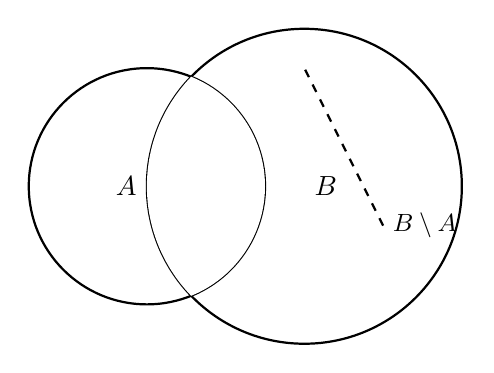
\begin{tikzpicture}
    % Conjunto A
    \draw[thick] (-1,0) circle (1.5) node[left] {$A$};
    % Conjunto B
    \draw[thick] (1,0) circle (2) node[right] {$B$};
    % Región B \ A (parte sombreada)
    \begin{scope}
      \clip (-1,0) circle (1.5);
      \fill[white] (1,0) circle (2);
    \end{scope}
    \draw[dashed, thick] (2, -0.5) -- (1, 1.5);
    \node[right] at (2, -0.5) {\small $B \setminus A$};
  \end{tikzpicture}
}
  \caption{$A \cup B = A \cup (B \setminus A)$}
\end{figure}

\begin{figure}[h]
  \centering
  \foreignlanguage{english}{
  \begin{tikzpicture}
    % Conjunto A
    \draw[thick] (-1,0) circle (1.5) node[left] {$A$};
    % Conjunto B
    \draw[thick] (1,0) circle (2) node[right] {$B$};

    % Región A ∩ B (parte sombreada)
    \begin{scope}
      \clip (-1,0) circle (1.5);
      \fill[pattern=north west lines] (1,0) circle (2);
    \end{scope}

    % Región B \ A (parte sombreada diferente)
    \begin{scope}
      \clip (1,0) circle (2);
      \fill[white] (-1,0) circle (1.5);
    \end{scope}

    \draw[dashed, thick] (1.8, -0.3) -- (2.5, -0.3);
    \node[right] at (2.5, -0.3) {\small $B \setminus A$};

    \draw[dashed, thick] (0, -1) -- (-0.5, -1.5);
    \node[left] at (-0.5, -1.5) {\small $A \cap B$};
  \end{tikzpicture}
}
  \caption{$B = (B \setminus A) \cup (A \cap B)$}
\end{figure}

Proposición. Sean $A$ y $B$ dos conjuntos finitos. Entonces, $A \times B$ es
un conjunto finito y 

$$ \text{card}(A \times B) = \text{card}(A) \cdot \text{card}(B) $$

Demostración. Supongamos que $A \neq \emptyset$ y $B \neq \emptyset$
pues en caso contrario la fórmula es trivial. Procedemos por inducción sobre
el cardinal de $B$.

Si $\text{card}(B) = 1$ entonces $B = \{b\}$ y $A \times B = A \times \{b\}$
que es equipotente con el conjunto $A$.

Supuesto que $\text{card}(A \times B') = \text{card}(A) \cdot
\text{card}(B')$ para todo conjunto $B'$ tal que $\text{card}(B') = n$, sean
$B$ tal que $\text{card}(B) = n + 1$ y $b \in B$. Consideramos el conjunto
$B' = B \setminus \{b\}$. Como $A \times B = A \times (B' \cup \{b\}) = (A
\times B') \cup (A \times \{b\})$, con $(A \times B') \cap (A \times \{b\})
= \emptyset$, por la proposición 5.15 y la hipótesis de inducción se
obtiene:

$$
  \begin{aligned}
    \text{card}(A \times B)
      &= \text{card}(A \times B') + \text{card}(A \times \{b\}) \\
      &= \text{card}(A) \cdot n + \text{card}(A) \\
      &= \text{card}(A) \cdot (n + 1)
  \end{aligned}
$$

Proposición. Sean $A$ y $B$ dos conjuntos finitos. Supongamos que $a =
\text{card}(A) \neq 0$ y $b = \text{card}(B) \neq 0$. Entonces, el número de
aplicaciones de $A$ en $B$ es $b^a$. Es decir:

$$ \text{card} \left( \mathcal{F}(A,B) \right) = \text{card} \left( B^A
\right) = b^a $$

Demostración. Se procede por inducción sobre $a$.

Para $a = 1$, dado que una aplicación de $A$ a $B$ está determinada por la
imagen del único elemento de $A$, existen tantas aplicaciones como elementos
hay en $B$, esto es $\text{card}(B^A) = b$.

Supongamos que $\text{card}(B^A) = b^a$ si $\text{card}(A) = a$ y sea $A' =
A \cup \{q\}$ con $q \notin A$. Así pues $\text{card}(A') = a + 1$. Veamos
que $\text{card}(B^{A'}) = b^{a+1}$. En efecto, dada una aplicación de $A$
en $B$, ésta se puede extender a una aplicación de $A'$ a $B$ dando la
imagen del elemento $q$. Como hay $b$ valores posibles para la imagen del
elemento $q$, por cada aplicación de $A$ a $B$ obtenemos $b$ aplicaciones
distintas de $A'$ a $B$. Dos extensiones a $A'$ de dos aplicaciones
distintas de $A$ a $B$ son obviamente distintas. Además, cualquier
aplicación de $A'$ a $B$ es una extensión de una aplicación de $A$ a $B$.
Por tanto:

$$ \text{card}(B^{A'}) = b \cdot \text{card}(B^A) = b \cdot b^a = b^{a+1} $$

Observación. La fórmula anterior sigue siendo cierta si $a = 0$ o $b = 0$,
pero no simultáneamente nulos. Si $B = \varnothing$ y $A \neq \varnothing$
entonces $\mathcal{F}(A, \varnothing) = \varnothing$ y en consecuencia,
$\text{card} \left( \mathcal{F}(A, \varnothing) \right) = 0 = 0^a$ si $a
\neq 0$. Si $A = \varnothing$, entonces el conjunto $\varnothing$ es el
único subconjunto del producto cartesiano $A \times B = \varnothing$, y
además es una aplicación de $A$ a $B$ que se denomina \textit{aplicación
vacía}. En consecuencia, $\text{card} \left( \mathcal{F}(\varnothing, B)
\right) = 1$.

Ejercicio. ¿Cuántas apuestas sencillas distintas (resultados 1, X y 2 en
catorce encuentros de fútbol) se pueden hacer en una quiniela?

Solución. Basta observar que existe una biyeción entre el conjunto de
apuestas y el conjunto de aplicaciones del conjunto $A = \{1,2,3,\dots,14\}$
en el conjunto $B = \{1, X, 2\}$. Por tanto el número de apuestas posibles
es $3^{14}$.

Proposición. Sea $A$ un conjunto finito. Entonces, el número de subconjuntos
de $A$ es $2^{\text{card}(A)}$, es decir:

$$ \text{card} \left( \powset(A) \right) = 2^{\text{card}(A)} $$

Demostración. Basta observar que existe una aplicación biyectiva entre el
conjunto $\powset(A)$ de las partes del conjunto $A$ y el conjunto
$\mathcal{F}(A, \{0,1\})$ de las aplicaciones de $A$ en $\{0,1\}$ que asocia
a todo subconjunto $B$ de $A$ la función característica $\chi_B : A
\longrightarrow \{0,1\}$ tal que

$$
  \chi_B(x) =
  \begin{cases}
    1 & \text{si } x \in B \\
    0 & \text{si } x \in A \setminus B
  \end{cases}
$$

En consecuencia, $\text{card} \left( \powset(A) \right) = \text{card} \left(
\mathcal{F}(A, \{0,1\}) \right) = 2^{\text{card}(A)}$.

Sean $A$ y $B$ dos conjuntos. Designamos por $\mathcal{B}(A,B)$ al conjunto
de aplicaciones biyectivas de $A$ en $B$ y por $\mathcal{I}(A,B)$ al
conjunto de aplicaciones inyectivas de $A$ en $B$. Si $A$ y $B$ son
conjuntos finitos entonces $\mathcal{B}(A,B)$ y $\mathcal{I}(A,B)$ también
lo son pues ambos son subconjuntos del conjunto finito $\mathcal{F}(A,B)$.

Proposición. Sean $A$ y $B$ dos conjuntos finitos cuyos cardinales son
$\text{card}(A) = n \neq 0$ y $\text{card}(B) = m \neq 0$ con $n \leq m$.
Entonces el número de aplicaciones inyectivas de $A$ en $B$ es

$$ \text{card} \left( \mathcal{I}(A,B) \right) = m(m-1) \cdots (m-n+1) $$

\noindent es decir, es el producto de $n$ enteros consecutivos siendo $m$ el
mayor de ellos.

Demostración. Procedemos por inducción sobre $n$.

1. Si $n = 1$, toda aplicación de $A$ a $B$ es inyectiva y por tanto hay
$m^1 = m$ aplicaciones inyectivas.

2. Supongamos cierto para $n < m$, esto es, se cumple que $\text{card}
\left( \mathcal{I}(A,B) \right) = m(m-1)\cdots(m-n+1)$. Veámoslo para $n+1$.
Sea $A' = A \cup \{c\}$ con $c \notin A$ y por tanto, $\text{card}(A') =
n+1$. Veamos que $\text{card} \left( \mathcal{I}(A', B) \right) =
m(m-1)\cdots(m-n)$.

En efecto, una aplicación inyectiva de $A$ a $B$ se puede extender a una
aplicación de $A'$ a $B$ dando la imagen del elemento $c$. Como hay $n$
elementos de $B$ que ya son la imagen de algún elemento de $A$, hay $m-n$
valores posibles para la imagen del elemento $c$ y en consecuencia, por cada
aplicación inyectiva de $A$ a $B$ obtenemos $m-n$ aplicaciones inyectivas
distintas de $A'$ a $B$. Dos extensiones a $A'$ de dos aplicaciones
distintas de $A$ a $B$ son obviamente distintas. Además, cualquier
aplicación inyectiva de $A'$ a $B$ es una extensión de una aplicación
inyectiva de $A$ a $B$. Por tanto:

$$ \text{card} \left( \mathcal{I}(A', B) \right) = (m-n) \cdot \text{card}
\left( \mathcal{I}(A, B) \right) $$

$$ = (m-n) \cdot m(m-1)\cdots(m-n+1) $$

$$ = m(m-1)\cdots(m-n) $$

Observación. El número $m(m-1)\cdots(m-n+1)$ se denota por $V_{m,n}$ y se
lee como \emph{variaciones de $m$ sobre $n$}. Es fácil comprobar que:

$$ V_{m,n} = m(m-1)\cdots(m-n+1) = \frac{m!}{(m-n)!} $$

Cuando $\text{card}(A) = \text{card}(B)$ sabemos que toda aplicación
inyectiva es biyectiva. Como consecuencia inmediata se obtiene la siguiente
proposición:

Proposición. Sean $A$ y $B$ dos conjuntos finitos tales que $\text{card}(A)
= \text{card}(B) = n$. Entonces el número de aplicaciones biyectivas de $A$
sobre $B$ es:

$$ \text{card} \left( \mathcal{B}(A, B) \right) = n! $$

Finalmente indicamos el número de subconjuntos de $n$ elementos que se
pueden extraer de un conjunto de $m$ elementos. Hágase la demostración a
modo de ejercicio.

Proposición. Sea $A$ un conjunto finito tal que $\text{card}(A) = m$. Sea $0
\leq n \leq m$. El número de subconjuntos de $A$ que poseen exactamente $n$
elementos es:

$$ \binom{m}{n} $$

Observación. El número $\binom{m}{n}$, que se lee \textbf{m sobre n}, se
denomina \emph{coeficiente binómico} o \emph{número combinatorio}. Se denota
también por $C_{m,n}$ y se lee \textbf{combinaciones de $m$ sobre $n$}.

Ejemplo. Interpretación teórica de la fórmula \quad $\binom{m}{n} =
\binom{m}{m-n}$ \quad si \quad $0 \leq n \leq m$.

La fórmula anterior es evidente si se utiliza la expresión

$$ \binom{m}{n} = \frac{m!}{n!(m-n)!} $$

Conceptualmente es también sencilla de establecer: la aplicación $f:
\powset(A) \longrightarrow \powset(A)$ tal que $f(B) = CB = A \setminus B$
es una biyeción. En particular, establece una biyeción entre el conjunto de
subconjuntos de $n$ elementos con el conjunto de subconjuntos de $m-n$
elementos.

Ejercicio. ¿Cuántas diagonales tiene un polígono convexo de $n$ lados?

Solución. Cada dos vértices no consecutivos del polígono obtenemos una
diagonal. Con dos vértices consecutivos se obtiene un lado del polígono.
Tenemos $n$ vértices posibles. En consecuencia, el número de subconjuntos de
2 elementos que se pueden extraer del conjunto de los $n$ vértices es la
suma del número $x$ de diagonales más el número $n$ de lados. Luego $x =
\binom{n}{2} - n$.














